%
\chapter{Metodologia}
\label{chap:metodologia}

\section{Descrição do Processo} \label{sec:descricaoprocesso}

Como já mencionado no \autoref{chap:introduction}, o processo modelado
neste trabalho utilizou os dados publicados por \citeonline{Rojas2014a}. 

\subsection{Diagrama Esquemático} \label{sec:diagramaesquematico}

O reator é composto de dois leitos catalíticos, carregados de forma densa
(\emph{dense loading}). No topo de ambos os leitos há catalisador carregado de
forma solta (\emph{sock loading}). A carga é composta de gasolina de pirólise,
hidrogênio e parte do produto hidrogenado reciclado. Este último é parte da
corrente líquida oriunda de um vaso de separação, cuja carga é a corrente de
saída do reator. Parte da corrente líquida do vaso de separação também
funciona como corrente de resfriamento, que é injetada entre os dois leitos
catalíticos para controle de temperatura. Um diagrama simplificado que ilustra o
reator está na \autoref{fig:esquemareator}. A \autoref{tab:dadosreator}
apresenta as dimensões do reator.

\begin{figure}[htb]
\centering 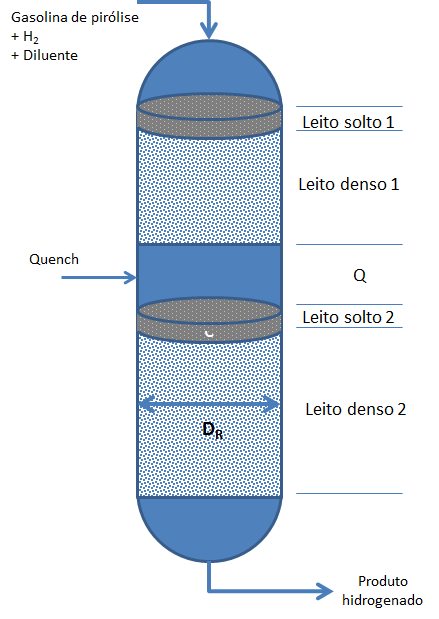
\includegraphics[scale=0.75]{images/Chap3/esquemareator.png}
\caption{Diagrama esquemático do reator \cite{Rojas2014a}.}
\label{fig:esquemareator}
\end{figure}


\begin{table}[!htb]
\begin{center}
\caption{Dados do Reator \cite{Rojas2014a}.}
\label{tab:dadosreator}
\small
\begin{tabular}{cc}
{Dimensão} & {Valor}
\\
\hline
{Diâmetro do Reator ($D_R$)} & $3,047$ m \\
{Leito Solto 1 ($L_{sl1}$)} & $0,13$ m \\
{Leito Denso 1 ($L_{dl1}$)} & $2,97$ m \\
{Leito Solto 2 ($L_{sl2}$)} & $0,38$ m \\
{Leito Denso 2 ($L_{dl2}$)} & $2,97$ m \\
{Zona de Quench ($L_{q}$)} & $1,55$ m \\
\bottomrule
\end{tabular}
\end{center}
\end{table}

\nomenclature{$L_{sl1}$}{Comprimento do leito solto 1 \nomunit{m}}
\nomenclature{$L_{dl1}$}{Comprimento do leito denso 1 \nomunit{m}}
\nomenclature{$L_{sl2}$}{Comprimento do leito solto 2 \nomunit{m}}
\nomenclature{$L_{dl2}$}{Comprimento do leito denso 2 \nomunit{m}}
\nomenclature{$L_{q}$}{Comprimento da zona de quench \nomunit{m}}

\subsection{Composição das Correntes} \label{sec:composicaocorrentes}

A composição das correntes de entrada e de quench estão na
\autoref{tab:composicao}. Para o presente trabalho, utilizou-se
apenas os valores da primeira corrida publicados por
\citeonline{Rojas2014a}, já que para essa corrida foram publicados
também dados industriais. Percebe-se pela composição que a gasolina de pirólise
é uma mistura bastante complexa.

As propriedades termodinâmicas dos compostos $28$ e $29$ não foram
encontradas. Assim, eles foram considerados como sendo parte dos compostos
$26$ e $27$, respectivamente.

\begin{table}[!htb]
\begin{center}
\caption{Composição das correntes de entrada e de quench \cite{Rojas2014a}.}
\label{tab:composicao}
\small
\begin{tabular}{clcc}
{Identificador $i$} & {Composto} & {$w$}\%  Entrada & {$w$}\%  Quench
\\
\hline
1 & Hidrogênio				& $0,48$ & $0,08$ \\
2 & Metano					& $0,52$ & $0,70$ \\
3 & Etano					& $0,12$ & $0,11$ \\
4 & n-Propano				& $0,36$ & $0,27$ \\
5 & n-Butano				& $0,30$ & $0,24$ \\
6 & n-Pentano				& $5,40$ & $5,60$ \\
7 & trans-2-Penteno			& $5,30$ & $7,60$\\
8 & trans-1,3-Pentadieno	& $2,50$ & $0,23$ \\
9 & Ciclopentano			& $1,50$ & $2,60$ \\
10& Ciclopenteno			& $2,10$ & $3,00$ \\
11& Metil-1,3-Ciclopentadieno	& $1,90$ & $0,21$ \\
12& n-Hexano				& $3,30$ & $3,30$ \\
13& Metilciclopentano		& $1,60$ & $1,70$ \\
14& Metilciclopenteno		& $2,00$ & $2,60$ \\
15& 1,3-Ciclopentadieno		& $1,90$ & $0,02$ \\
16& Benzeno					& $28,90$ & $30,10$ \\
17& n-Heptano				& $2,80$ & $2,90$ \\
18& Tolueno					& $16,00$ & $16,30$ \\
19& n-Octano				& $1,30$ & $1,30$ \\
20& Etilbenzeno				& $3,40$ & $5,40$ \\
21& Estireno				& $2,00$ & $0,11$ \\
22& Xileno					& $5,40$ & $5,50$ \\
23& n-Nonano				& $0,66$ & $0,72$ \\
24& 1-Metil-3-Etilbenzeno	& $2,90$ & $3,90$ \\
25& Metilestireno			& $1,40$ & $0,31$ \\
26& Dihidrodiciclopentadieno	& $1,80$ & $3,00$ \\
27& Diciclopentadieno		& $1,80$ & $0,12$ \\
28& Metildihidrodiciclopentadieno	& $1,50$ & $2,20$ \\
29& Metildiciclopentadieno	& $0,88$ & $0,11$ \\
\bottomrule
\end{tabular}
\end{center}
Onde $i$ é o número identificador do composto na simulação a ser apresentada.
\end{table}

\nomenclature[S]{$i$}{i-ésimo componente \nomunit{m}}

\section{Premissas} \label{sec:premissas}

Antes de apresentar as premissas que nortearam o presente trabalho, vale
aqui definir, para efeito de comparação, as premissas utilizadas por
\citeonline{Rojas2014a}.

\begin{enumerate}
  \item O reator opera em estado estacionário e adiabaticamente.
  \item Gradientes radiais são desprezíveis.
  \item Dispersões axiais foram negligenciadas; portanto, assumiu-se o
  escoamento empistonado para ambas as fases líquida e gasosa.
  \item A fase gasosa está em excesso; dessa forma, negligenciou-se a
  resistência a transferência de massa na fase gasosa.
  \item Fator de molhamento, atividade catalítica e densidade do leito
  uniformes.
  \item A transferência de calor entre as fases e no interior das partículas de
  catalisador foram desprezadas.
  \item A região do quench é assumida como sendo um tambor flash, que atinge o
  equilíbrio instantaneamente.
  \item A corrente de saída do primeiro leito mistura-se instantaneamente com a
  corrente de quench.
  \item O reator opera em regime de bolha.
  \item Reações reversíveis e isomerizações foram negligenciadas.
  \item As reações ocorrem somente na interface líquido-sólido.
  \item A desativação catalítica foi desprezada.
\end{enumerate}

